\documentclass[a4paper,12pt]{report}
\usepackage{listings}
\usepackage[utf8]{inputenc}
\usepackage{import}
\usepackage[utf8]{inputenc}
\usepackage{textcomp}
\usepackage{float}
\usepackage{subfig}
\usepackage{mathtools}
\usepackage{setspace}
\usepackage{graphicx}
\usepackage{graphics}
\usepackage{epstopdf}

%\usepackage[spanish,es-tabla]{babel}
%\usepackage[nottoc,numbib]{tocbibind}
\renewcommand{\baselinestretch}{1.5}
%caracteristicas de paginas
\pdfpagewidth 8.5in
\pdfpageheight 11in
\setlength\oddsidemargin{-0,21in}
\setlength\evensidemargin{-0,21in}
\setlength\topmargin{-2cm}
\setlength\textwidth{7in}
\setlength\textheight{23.7cm}
\setlength\parskip{0.1in}
\def\thechapter{\arabic{chapter}}
\renewcommand{\chaptername}{Capítulo}
\renewcommand{\contentsname}{Contenidos}
\renewcommand\bibname{Bibliografía}

% Biblio: http://www.csse.monash.edu.au/documents/bibtex/

\begin{document} 

\thispagestyle{empty}

\begin{center}

% Parte Superior
 \begin{figure}[htb]
\centering

\includegraphics[width=0.45\textwidth]{caratula/logo.png}
\end{figure} 



\textsc{\LARGE Universidad de Buenos Aires}\\[0.5cm]
\textsc{\large Facultad de Ciencias Exactas y Naturales}\\[0.5cm]

\textsc{  Departamento de Física Juan José Giambiagi}\\[0.5cm]


% Titulo
%\HRule \\[0.4cm]
\huge Dinámica de partículas autoimpulsadas: evacuación a través de dos puertas.\\
%\HRule \\[1cm]

\textsc{\large Tesis de Licenciatura}\\[1cm]

% Autores y Directores
{\LARGE \textbf{
Ignacio Mariano Sticco}} \\ [1cm]

\large
Director: Dr. Claudio Oscar Dorso \\[0.5cm]
Codirector: Dr. Guillermo Alberto Frank
\vfill

% Parte Inferior

 Septiembre de 2016

\end{center}

\newpage


\begin{flushleft}
TEMA: Título de la tesis\\

ALUMNO: Ignacio Mariano Sticco\\

LU N$^{\circ}$: 888/10 \\

LUGAR DE TRABAJO: Departamento de Física, Consejo Nacional de Investigaciones Cient\'ificas y T\'ecnicas (CONICET) - Universidad de Buenos Aires (UBA)\\

DIRECTOR DEL TRABAJO: Dr. Claudio Oscar Dorso \\

CODIRECTOR DEL TRABAJO: Dr. Guillermo Alberto Frank\\

FECHA DE INICIACI\'ON: Septiembre de 2015 \\

FECHA DE FINALIZACI\'ON: Septiembre de 2016\\

FECHA DE EXAMEN:  \\

INFORME FINAL APROBADO POR:
\end{flushleft}                                                              %
                                                            %
\vspace{2cm}

\begin{center}
\begin{tabular}{|c|c|}
\hline
Autor &  \,\,\,\,\, \,\,\,\,\,\,\,\,\, \,\,\,\,\,\,\,\,\,\,\,\,\,\,\,\,\,\,Jurado \,\,\,\,\,\,\,\,\,\,\,\,\,\,\,\,\,\,\,\, \,\,\,\,\,\,\,\,\,\,\,\, \\
&            \\
       &            \\
  ..............................            &     ..............................          \\
       &            \\

\hline
Director &      \,\,\,\,\, \,\,\,\,\,\,\,\,\, \,\,\,\,\,\,\,\,\,\,\,\,\,\,\,\,\,\,Jurado \,\,\,\,\, \,\,\,\,\,\,\,\,\,\,\,\,\,\,\,\,\,\,\,\, \,\,\,\,\,\,\,\\
&            \\
       &            \\
  ..............................            &       ..............................        \\
         &            \\
 \hline
Profesor de Tesis de Licenciatura &  \,\,\,\,\,\,\, \,\,\,\,\, \,\,\,\,\,\,\,\,\,\,\,\,\,\,\,\,\,\,\,\,Jurado \,\,\,\,\,\,\,\,\,\,\,\,\,\,\,\,\,\,\,\,\,\,\,\,\,\,\, \,\,\,\,\,\\
&            \\
       &            \\
  ..............................            &      ..............................         \\
         &            \\
\hline
\end{tabular}
\end{center}

A mi codirector Guillermo Frank que con su vocación docente supo enseñarme las bases de la física computacional y contagiarme el entusiasmo por la labor del día a día. \\

A mi director Claudio Dorso que gracias a ese balance entre buen humor y exigencia logra que las cosas funcionen como deben. \\

A Pablo Alcaín, embajador de la buena programación, brindó muchísimo apoyo en esta investigación, sus consejos siempre van en la dirección correcta. \\

A Fernando Cornes, Guillermo Pascualetti y Sebastián Pinto, con quienes compartí almuerzos, espacio de trabajo e información valiosa. 

A mi papá y mi mamá que fomentan mi bienestar de innumerables maneras. A mi hermana Magui por sus charlas amenas y profundas a la vez. A mi hermano Patri, su colaboración fue clave para avanzar con algunos asuntos computacionales.\\

A mi abuela Ada, por todos esos almuerzos tan cargados de alegría como de comida deliciosa. A mi tía Meme quien me dio ánimos en momentos de desgano.\\

A mi abuelo Abel, siempre estimuló mi curiosidad y mucho tuvo que ver con mi incursión en la ciencia. \\

A mis amigos Hernan Martinelli e Ignacio Sallaberry, juntos desde el comienzo de la carrera. Por todos esos encuentros catárticos acompañadas de cerveza.\\ 

A mi amor Ana Rosso, compañera de charlas nerd, caminatas relajantes e infinitos momentos llenos de risas. Sin ella no tendría la paz que necesito para estar bien. 
\tableofcontents
\chapter{Introducción}
\section{Antecedentes}

La práctica de incluir dos puertas para evacuaciones de emergencia se remonta a los tiempos de la última dinastía Qing en China (1644-1911 AD). Existía una ley que establecía que los edificios grandes debían tener dos salidas para evitar problemas en caso de incendio~\cite{cheng}.
Los códigos estándar actuales cuantan con especificaciones detalladas de las ubicaciones de las puertas, el ancho y la separación entre éstas~\cite{OSHA,FLO}.
 
Las reglamentaciones actuales exigen que el ancho mínimo de las puertas debe ser 0,813~m y el tamaño máximo de una hoja no debe ser mayor a 1,219~m\cite{FLO,FLO2}. Si se requieren más de dos puertas, la separación entre dos de ellas debe ser al menos un cuarto o un tercio de la distancia diagonal de la habitación. No hay ningún requerimiento especial sobre el resto de las puertas, más alla del hecho que no deben estar simultaneamente bloqueadas\cite{FLO,FLO2}.\\

La reglamentación da lugar a ubicar las salidas adicionales (\emph{i.e.} las puertas arriba mencionadas) con una distancia de separación arbitraria. De esta forma, se pueden ubicar dos puertas en un mismo flanco del cuarto. El caso especial de dos puertas contiguas ha sido examinado en la literatura~\cite{kirchner1,perez1,daoliang1,huanhuan1}. \\

Kirchner y Schadschneider estudiaron el proceso de evacuación de peatones a través de dos puertas contiguas usando un modelo de autómatas celulares\cite{kirchner1}. Los agentes podían abandonar la habitación con comportamientos que iban desde el individualismo hasta un movimiento fuertemente acoplado como el de una \emph{manada}. Se encontró que el tiempo de evacuación es independiente de la distancia de separacipón para el caso de peatones con comportamiento individualista. Pero, si los peatones se movían en manada, se reportó un tiempo de evacuación mayor para pequeñas separaciones (menores al tamaño de 10 individuos).\\

El número de peatones que abandonó el recinto por unidad de tiempo mostró una disminución para distancias de separación menores al ancho de cuatro puertas\cite{perez1}. Esta disminución del flujo fue asociada a un efecto de interferencia debido a peatones cruzandose mutuamente. El umbral de cuatro anchos de puerta ($4\,d_w$) corresponde a la distancia de separación necesaria para distinguir dos  grupos independientes de peatones, cada uno de ellos rodeando a la puerta más cercana. \\

Los investigadores destacaron el hecho que no importa cuan separadas estén las dos puertas, el rendimiento de la evacuación no mejora el doble respecto al rendimiento que tiene una única salida (con el mismo ancho). Este efecto se le atribuye a algún tipo de interferencia entre peatones\cite{perez1}.\\

Aunque los resultados arriba mencionados fueron obtenidos para puertas muy angostas (\emph{i.e.} del ancho de un individuo), investigaciones posteriores mostraron que también aplican a puertas que permiten el paso de dos peatones. Sin embargo, esto no aplica a habitaciones con una única puerta\cite{daoliang1}. En este caso, el flujo medio de peatones evacuados aumenta con el ancho de la puerta, pero el flujo por unidad de ancho decrese\cite{daoliang1}. \\
 
El rendimiento de la evacuación puede verse afectado por la distancia de separación de las puertas si éstas estan ubicadas cerca de una pared, es decir, cerca de la esquina del cuarto. La gente entra en contacto con las paredes, perdiendo eficiencia en la evacuación\cite{kirchner1,daoliang1}. \\

Investigaciones más detalladas con automatas celulares mostraron que el rendimiento en la evacuación depende de cinco longitudes: el ancho total de las salida (es decir, sumar los anchos de cada puerta), la distancia de separación entre puertas, la diferencia de ancho entre las puertas y la distancia a la esquina más cercana \cite{huanhuan1}. \\

El ancho total de las salidas puede mejorar el tiempo de evacuación para cualquier distancia de separación entre puertas, siempre que ambas tengan el mismo ancho. 
Sin embargo, la separación controla la ubicación óptima para
estas salidas. A grandes rasgos, la distancia de separación $d_g$ debe ser igual a $L-4\,d_w$, donde $L$ es la longitud del cuarto\cite{huanhuan1}. \\

La ubicación optima concuerda con el fenómeno de disminución del flujo para pequeños valores de $d_g$. También se condice con el empeoramiento del rendimiento de la evacuación para puertas cercanas a la esquina. Pero esta disminución puede surgir por otras razones, ya que el aumento del recorrido de los peatones a las puertas juega un papel importante.\\ 

La configuración con dos puertas no necesita ser simétrica a lo largo de la pared. La asimetría provoca demoras que dependen de la diferencia del ancho de las puertas y sus posiciones relativas. Ubicar a la puerta más ancha en el medio de la pared y a la menor en la esquina, ocasiona un mejora en el proceso de evacuación\cite{huanhuan1}.\\

Esta investigación se centra en configuraciones simétricas con puertas de igual tamaño. A diferencia de la literatura arriba mencionada, se examina la dinámica de la evacuación a través del modelo de fuerza social. En el capítulo siguiente se encuentra una descripción de este modelo. \\

\newpage

\section{Objetivos}

En este trabajo nos proponemos estudiar la dinámica de multitudes evacuando en estado de  pánico en recintos con una o dos puertas.\\ 

Se compararán campos de presión y velocidad para recintos con puertas anchas y angostas.\\

Se modificará la cantidad de peatones y el grado de ansiedad de los individuos para observar cómo estas propiedades alteran la dinámica y encotrar magnitudes que sean independientes de las mismas.\\

Se realizarán simulaciones para saber a qué distancia deben ubicarse las puertas para que la evacuación se efectúe en el menor tiempo posible.



\chapter{Marco Teórico}
En este capítulo se describirá el modelo en el cual se basa toda la investigación, también se definirán los conceptos utilizados a lo largo del trabajo como la definición de la presión social y los blocking clusters. Además se comentará el algoritmo de Verlet, ya que fue utilizado para resolver la dinámica del problema. 

\section{\label{sfm}Modelo de Fuerza social}

El modelo de fuerza social es un modelo basado en agentes utilizado para simular el movimiento de peatones. Supone que los individuos soportan tres tipos de fuerzas: fuerzas de deseo (autopropulsión), sociales (repulsión) y granulares (rozamiento).  \\

La fuerza de autopropulsión refleja el hecho que el individuo i-esimo que posee masa $m_i$, desea  moverse con una velocidad $v_d^ {(i)}(t)$ en una dirección $\hat{\mathbf{e}}_d^ {(i)}(t)$, por lo tanto readapta su velocidad $\mathbf{v}_i(t)$ con un cierto tiempo característico $\tau$.
\begin{equation}
\mathbf{f}_d^ {(i)}(t)=m_i\,\displaystyle\frac{v_d^ {(i)}(t)\,\hat{\mathbf{e}}_d^ {(i)}(t)-\mathbf{v}_i(t)}{\tau}\label{fdeseo}
\end{equation}

La repulsión social es una fuerza que describe la tendencia que tienen las personas a mantenerse alejadas unas de otras. Depende de la distancia de separación entre individuos $d_{ij}=\left\|\mathbf{r_i}-\mathbf{r_j}\right\|$ y está en la dirección normal $\mathbf{n}_{ij}=(n_{ij}^1,n_{ij}^2)/d_{ij}$ (versor que apunta desde el individuo j al individuo i). Los peatones están en contacto si el valor de $d_{ij}$ es más chico que la suma de los radios $r_{ij}=(r_i+r_j)$. $A_i$ y 	$B_i$ son constantes.

\begin{equation}
\mathbf{f}_s^{(ij)}=A_i\,e^{(r_{ij}-d_{ij})/B_i}\mathbf{n}_{ij}\label{fsocial}
\end{equation} 

Cuando los individuos están en contacto, comienza a actuar una fuerza de rozamiento, la misma es proporcional a la velocidad relativa entre los mismos.  
$\Delta \mathbf{v}_{ij}=(\mathbf{v}_i-\mathbf{v}_j)$, la dirección tangencial está representada por $\mathbf{t}_{ij}=(-n_{ij}^2,n_{ij}^1)$.  $\kappa$ es una constante y $g(x)$ es una función nula cuando los individuos no se tocan $(r_{ij}<d_{ij})$ y toma el valor de su argumento en caso contrario. 
\begin{equation}
\mathbf{f}_g^{(ij)}=\kappa\,g(r_{ij}-d_{ij})\,\Delta \mathbf{v}_{ij}\cdot\mathbf{t}_{ij}\label{frozamiento}
\end{equation}

Se trata de forma análoga a la interacción de los individuos con las paredes. $d_{iW}$ es la distancia del i-esimo peatón con la pared W, $n_{iW}$ la dirección perpendicular entre éstos y $t_{iW}$ la tangencial. La expresión \ref{fparedes} agrupa tanto a la repulsión como al rozamiento de la interacción peatón-pared.

\begin{equation}
\mathbf{f}^{iW}=A_ie^{(r_{i}-d_{iW})/B_i}\mathbf{n}_{iW}-\kappa g(r_{i}-d_{iW})\Delta \mathbf{v}_{i}\cdot\mathbf{t}_{iW}
\label{fparedes}
\end{equation} 

Con todo esto, mediante la fórmula \ref{newton}, puede expresarse la variación de velocidad en el tiempo que siente un individuo. $f^{ij}$ es el término de interacción entre individuos, es la suma de la repulsión y el rozamiento. El cambio de posición viene dado por $v_{i}(t)=d\mathbf{r_i}/dt$.

\begin{equation}
m_i\frac{d\mathbf{v_i}}{dt}=\mathbf{f}_d^ {(i)}(t)+ \sum_{i\neq j}^{N}\mathbf{f}^{(ij)} + \sum_{W}^{N}\mathbf{f}^{(iW)}
\label{newton}
\end{equation}  

Uno de los resultados más trascendentes de este modelo es el efecto "Faster is slower" \cite{Helbing1}. A partir de cierto grado de apuro ($v_d=2$~m/s) un incremento en la velocidad de deseo produce evacuaciones menos eficientes (los peatones tardan más en evacuar). 
 
\section{Presión local}

A pesar de que la fuerza de deseo $\mathbf{f}_d$ y la fuerza social $\mathbf{f}_s$, del modelo de fuerza social, no son magnitudes "Físicas" (\textit{i.e.} no tienen par de reacción), la ecuación de movimiento sigue siendo válida. Por lo tanto, se puede derivar la relación del virial\cite{lion}. 

\begin{equation}
 \bigg\langle\displaystyle\sum_{i=1}^N\displaystyle\frac{p_i^2}{m_i} + 
\displaystyle\sum_{i=1}^N 
\mathbf{r}_i\cdot\mathbf{f}_i\bigg\rangle=0\label{virial1}
\end{equation}


\noindent Para un conjunto de $N$ pedestrians. $p_i$  y $\mathbf{f}_i$ son el impulso y la fuerza total actuando sobre el individuo $i$. $\langle\cdot\rangle$ corresponde al valor medio en el tiempo.  \\

La presión local para un peatón ($i$) está asociada a las fuerzas (por unidad de área) actuando sobre él debidas a los individuos que lo rodean y las paredes. Según Ref.~\cite{lion} se puede definir la "función de presión social" $P_i$ como:\\

\begin{equation}
3P_iV_i=\displaystyle\frac{p_i^2}{m_i} + \frac{1}{2}
\displaystyle\sum_{j=1}^{N-1}
\mathbf{r}_{ij}\cdot\mathbf{f}_s^{(ij)}\label{pv}
\end{equation}

\noindent donde $V_i$ es el volumen que encierra al peatón $i$ y 
$\mathbf{r}_{ij}=\mathbf{r}_{i}-\mathbf{r}_j$. Cabe destacar que el producto interno $\mathbf{r}_{ij}\cdot\mathbf{f}_s^{(ij)}$ siempre es positivo debido a la repulsión y es igual al producto escalar $d_{ij}f_s^{(ij)}$.  \\ 

El segundo término en la equación \ref{virial1} puede dividirse en la suma de productos internos $\mathbf{r}_i\cdot\mathbf{f}_d$ (deseo), 
$\mathbf{r}_i\cdot\mathbf{f}_s$ (social) y $\mathbf{r}_i\cdot\mathbf{f}_g$ (granular). De hecho, la suma del producto social depende de la distancia entre partículas $d_{ij}f_s^{(ij)}$, mientras que la parte granular no tiene ningún rol por su ortogonalidad ($\mathbf{r}_{ij}\cdot\mathbf{f}_g^{(ij)}=0$). Por lo tanto, la relación del virial (\ref{virial1}) se expresa \\  


\begin{equation}
 \displaystyle\sum_{i=1}^N\langle3P_iV_i 
\rangle=-\displaystyle\sum_{i=1}^N \langle
\mathbf{r}_i\cdot\mathbf{f}_d^{(i)}\rangle\label{virial2}
\end{equation}

Hay que destacar que la ecuación (\ref{virial2}) se cumple si los peatones están en contacto o no. La "función de presión social" $P_i$ hace que los individuos puedan cambiar su patrón de comportamiento cuando se acercan mucho unos con otros o con las paredes. \\ 


\section{Blocking Clusters}

Se utilizó el concepto de blocking cluster~\cite{Dorso1} para estudiar a los individuos más cercanos a la salida. Se lo define como un conjunto de individuos en contacto que va desde un punto de la pared hacia otro. Estos puntos están próximos a los costados de la puerta. Aquellos peatones que conforman el blocking cluster son los responsables de bloquear la salida. Típicamente los blocking cluster formados en las evacuaciones tiene estructura de "arco" como el que se muestra en la figura \ref{bc}. Basta que un solo peatón deje de estar en contacto con sus vecinos para que el blocking cluster deje de estar constituído. \\

\begin{figure}[H]
    \centering
    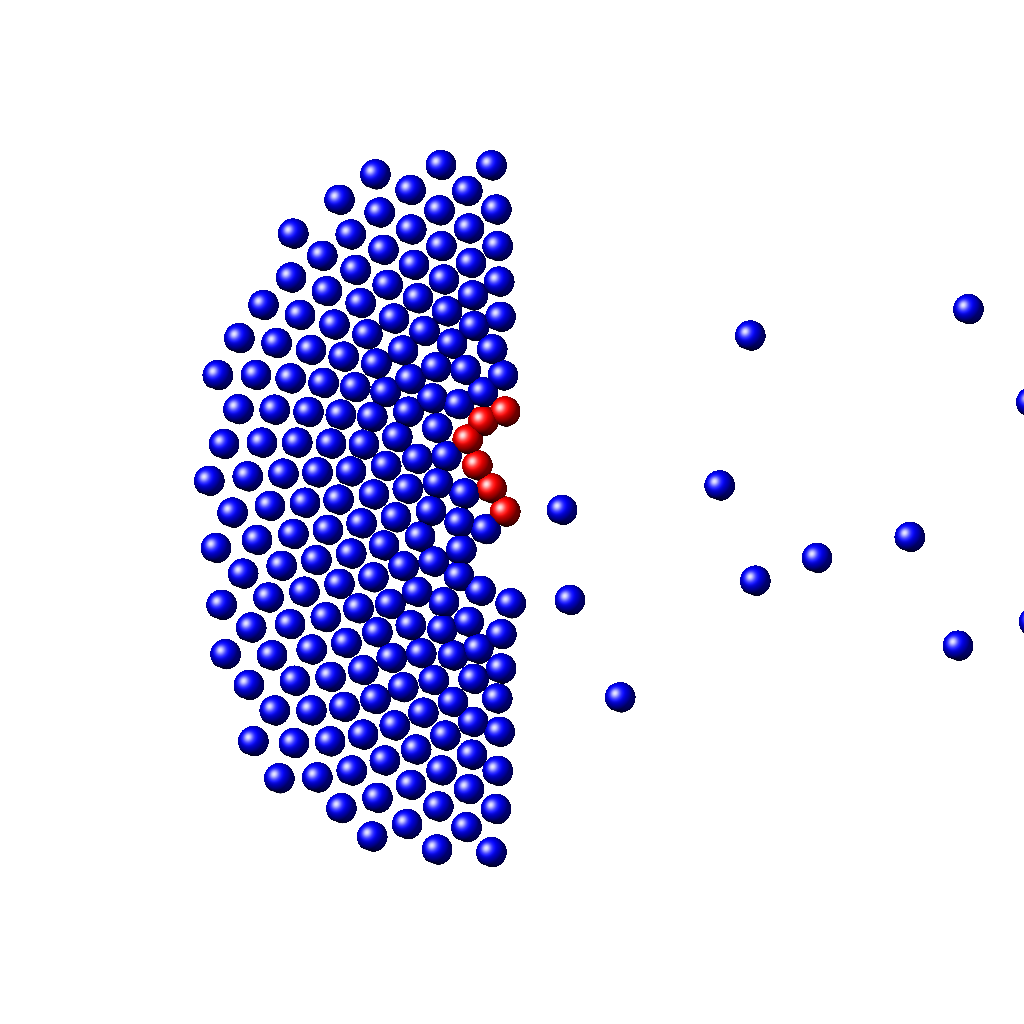
\includegraphics[height=5.5cm]{figuras/in_image_2_120000_bkg.png}
    \caption[width=5cm]{}
    \label{bc}
\end{figure}

A lo largo del trabajo se han usado dos tipos de blocking clusters: Big blocking cluster y small blocking cluster. El primero se tiene cuando hay dos puertas sobre la misma pared, son los individuos que van desde una puerta hasta la otra (encierran las dos salidas). El segundo es el bloqueo de una única salida. 

\section{Algoritmo de Verlet}

Para integrar las ecuaciones de movimiento se usó el algoritmo de Verlet, este método es ampliamente utilizado en el campo de dinámica molecular.\\
Este algoritmo es una combinación de dos expansiones de taylor sumadas para dar lugar a una expresión con términos pares únicamente~\cite{haile}

\begin{equation}
x(t+\Delta t)=2x(t)-x(t-\Delta t)+\frac{d^2x(t)}{dt^2} \Delta t^2+O(\Delta t^4)
\label{verlet_x}
\end{equation} 
Este es el algoritmo de Verlet para posiciones. Tiene un error de truncamiento local de ($\Delta^4$), por lo tanto es de tercer orden aunque no contenga derivadas de tercer orden. La aceleración es obtenida de fuerzas intermoleculares y la segunda ley de Newton.
Para estimar la velocidad se utiliza:
\begin{equation}
v(t)\simeq \frac{x(t+\Delta t)-x(t-\Delta t)}{2\Delta t}
\label{verlet_v}
\end{equation}
Para resolverlo se suelen llevar a cabo los siguientes pasos: se actualizan las velocidades, luego las posiciones, en tercer lugar las fuerzas y se vuelve a repetir el ciclo hasta completar las trayectorias. 
El algoritmo de Verlet posee buena estabilidad para pasos temporales moderadamente grandes.

\chapter{Simulaciones}

\noindent En este capítulo se describirán los métodos usados para llevar a cabo las simulaciones. 

\noindent Para realizar las simulaciones se utilizó el programa LAMMPS (Large-scale Atomic/Molecular Massively Parallel Simulator).
Es un software de código libre distribuido bajo los términos de GPL.
LAMMPS se caracteriza por hacer uso de las listas de vecinos [rapaport] para efecuar cálculos que permiten reducir la
complejidad algorítmica, además cuenta con una gran cantidad de funciones implementadas orientadas al uso de simulaciones
de dinámica molecular. 

\noindent Todas las simulaciones constaron de N individuos en un recinto cuadrado cuyo tamaño estaba ligado a la cantidad de
peatones de modo tal que mantenga constante la densidad. En una de las paredes se ubicó una o dos puertas dependiendo de qué 
se buscaba analizar.
Para todas los sistemas estudiados se configuró un arreglo bidimensional de individuos, ordenados inicialmente tipo
red cuadrada, separados entre si por una distancia de 1,3 m. La velocidad inicial se estipuló de modo que todos los individuos
tengan en promedio 1.7 m/s (en módulo) con una dispersion de m/s, la dirección fue generada aleatoriamente para
cada uno de ellos. Luego del instante inicial, los agentes cambiaban su velocidad acorde a la velocidad de deseo configurada 
(con el fin de que todos busquen evacuar la habitación). Una vez que los individuos abandonaban el recinto no se los reinyectaba.
De modo que al evacuar dejaba de importar sus observables. 
Para resolver la dinámica se utilizó el algoritmo de Verlet. 
\noindent Con el fin de compatibilizar el modelo de fuerza social con LAMMPS, se crearon varios módulos con las fuerzas que
caracterizan al modelo y algulas fnnciones que sirvieron para caracterizar al sistema. Todos estos fueron escritos en c++.

\section{Módulos}

{\Large pair\_social}

Este módulo se hizo para incluir la fuerza social del modelo de Helbing. Toma como parámetros la constante B y la distancia 
de corte (si los individuos estan separados por una distancia mayor a este corte, la fuerza social entre ellos no se calcula).
Otros parámetros son agregados a través de la función pair\_coef. Estos son la constante A del modelo de Helbing, la distancia 
de corte y el radio de los individuos. Los valores utilizados fueron: A $=$ 2000, B$=$ 0,08 r\_cut $=$ 3,5 d $=$ 0,30.
La elección de la distancia de corte se tomó de modo tal que la fuerza social que sienten individuos separados a esa distancia
sea despreciable ($\sim$ 10$^{-12}$). El resto de los parámetros se extrajeron de la bibliografia del modelo de fuerza social[].

{\Large pair\_gran\_social}

Se creó para que exista rozamiento entre los individuos que están en contacto. Requiere como parámetro el valor de la constante de rozamiento, el mismo fue $\kappa =$ 240000, tanto este valor como la expresión de la fuerza son acordes al modelo de Helbing.

{\Large fix\_wall\_social y fix\_wall\_gran}

Estos módulos son análogos a pair\_social y pair\_gran\_social pero aplicados a las fuerzas de interacción entre los individuos y las paredes. El primero simula la fuerza de repulsión y poseé los mismos parámetros que la repulsión entre individuos mientras que el segundo modela la fuerza de rozamiento dinámico. 

{\Large fix\_social\_self y fix\_social\_self\_multi}

La fuerza de deseo del modelo de Helbing fue simulada con estos módulos. El primero se usó para los recintos con una única puerta mientras que el segundo para recintos con dos. 
El primero requiere como parámetro la masa de los individuos y la velocidad de deseo. El target que tiene cada individuo, depende de la posición en donde se encuentre. Por cada puerta hay tres targets: superior, medio e inferior. El medio está ubicado en la mitad de la puerta, los otros 0,3 m por encima y por debajo.  Los individuos cuya posición en la coordenada 'y' sea mayor (menor) que el target superior (inferior) actualizan su velocidad para apuntar al target superior (inferior). Si se encuentran en medio de éstos, apuntan al centro de la puerta. 
Cuando se simularon recintos con dos puertas se usó fix$\_$social$\_$self$\_$multi, sus parámetros son: la masa de los individuos, la velocidad de deseo y el gap (la distancia de separación entre puertas). Si el gap es nulo, las dos puertas estan unidas (formando una única puerta ancha). En este caso, se establecen tres targets: el superior (inferior) 0.3 m debajo (encima) del final de la puerta superior (inferior). Los individuos que se encuentran en el medio apuntan al centro (al igual que en el caso de una única puerta).
Si el gap es no nulo, es decir, existe una porción de pared entre ambas puertas, la dirección de la velocidad de los individuos se actualiza de forma análoga al caso de una puerta. 

{\Large compute\_social\_pressure}

Calcula la presión que siente cada individuo debida a la interacción de repulsión social. Para cada timestep devuelve un vector con la pesión de cada uno. 

{\Large compute\_dijkstra\_atom}

Rotula con la misma etiqueta a todos los elementos que forman parte de un blocking cluster. Requiere como parámetro las posiciones en la coordenada 'y' de los puntos de origen y terminación del blocking cluster y la posición de la pared en la coordenada 'x'. Para cada timestep, devuelve un vector con un número no nulo para los individuos que forman el cluster de bloqueo y cero para los que no. 

\section{Script básico}

A modo de ejemplo se describirá un script de lammps que se hizo para simular 225 individuos en un recinto de 20x20 m. Este programa cuenta con dos ciclos for, uno recorre diferentes valores de velocidad de deseo y el otro (anidado) sirve para tener 30 simulaciones con diferentes velocidades iniciales.  
El programa devuelve un video de la simulación en formato mpg, un archivo txt con una tabla que indica $v_d$, numero de iteración y el tiempo para el cual evacuaron 159 individuos. 

\begin{verbatim}
# Pedestrians in a 2D box
variable vdmax equal 6
variable vd loop 1 ${vdmax}
label start_of_loop1

variable itermax equal 30
variable iter loop 1 ${itermax}
label start_of_loop2

# 		 intial conditions
dimension        2
boundary         f f p
units            si
atom_style       sphere
lattice          sq 1.3 origin 0.5 0.5 0.0
region           zona1 block 0 20 0 20 -1 1 units box
region           zona2 block 20.12 40 0 20 -1 1 units box
region           zona3 block 19 21 9.4 10.6 -1 1 units box
region           todas union 3 zona1 zona2 zona3
create_box       1 todas
create_atoms     1 region zona1
set              atom * mass 70.0
set              atom * diameter 0.6
velocity         all create 1e23 ${iter} dist gaussian
comm_modify      vel yes

#  Interaction potentials
pair_style   hybrid/overlay gran/social 0 0 0 240000 0 1 social 0.08 3.5
pair_coeff   * * social 2000 3.5 0.3
pair_coeff   * * gran/social
compute      ps all social_pressure/atom
dump         presion all custom 500 in_press_225p_v4_onedoor.txt c_ps x y
dump_modify  presion append  yes

#  boundary conditions
fix  walls all wall/region todas social 2000 0.08 3.5
fix  wallg all wall/region todas granular 240000 120000 0.001    
fix  target all social/self 70 ${vd} xy          

compute     1 all property/atom x
variable    out atom c_1>20.0
compute     mycompute all reduce sum v_out
variable    evacuados equal c_mycompute
#variable   ps atom c_ps

# visualize
#dump  3 all movie 200 in.movie_press_onedoor.mpg c_ps type &
#      axes yes 0.8 0.02 view 0 0 zoom 2 adiam 0.6

# run the process
atom_modify   sort 0 0.0
timestep      0.0001
fix           1 all nve/limit 0.001
thermo_style  custom step c_mycompute

#	ESTE ES EL LOOP DE UN PROCESO
variable nmax equal 20000
variable n loop ${nmax}
label start_of_loop3
run  500
if "${evacuados} > 159" then "jump SELF break"
variable t equal 0.05*$n
next n
jump SELF start_of_loop3
#	TERMINACION DEL PROCESO
label break
#print "${vd}  ${iter}  $t" append print.txt
clear
variable n delete
next iter
jump SELF start_of_loop2
#	TERMINACION DEL LOOP 2
clear
next vd
jump SELF start_of_loop1
\end{verbatim}



\chapter{Resultados y Discusión}
\section{Una puerta}

\subsubsection{Puerta ancha (3,6 m)}

\begin{figure}[H]
    \centering
    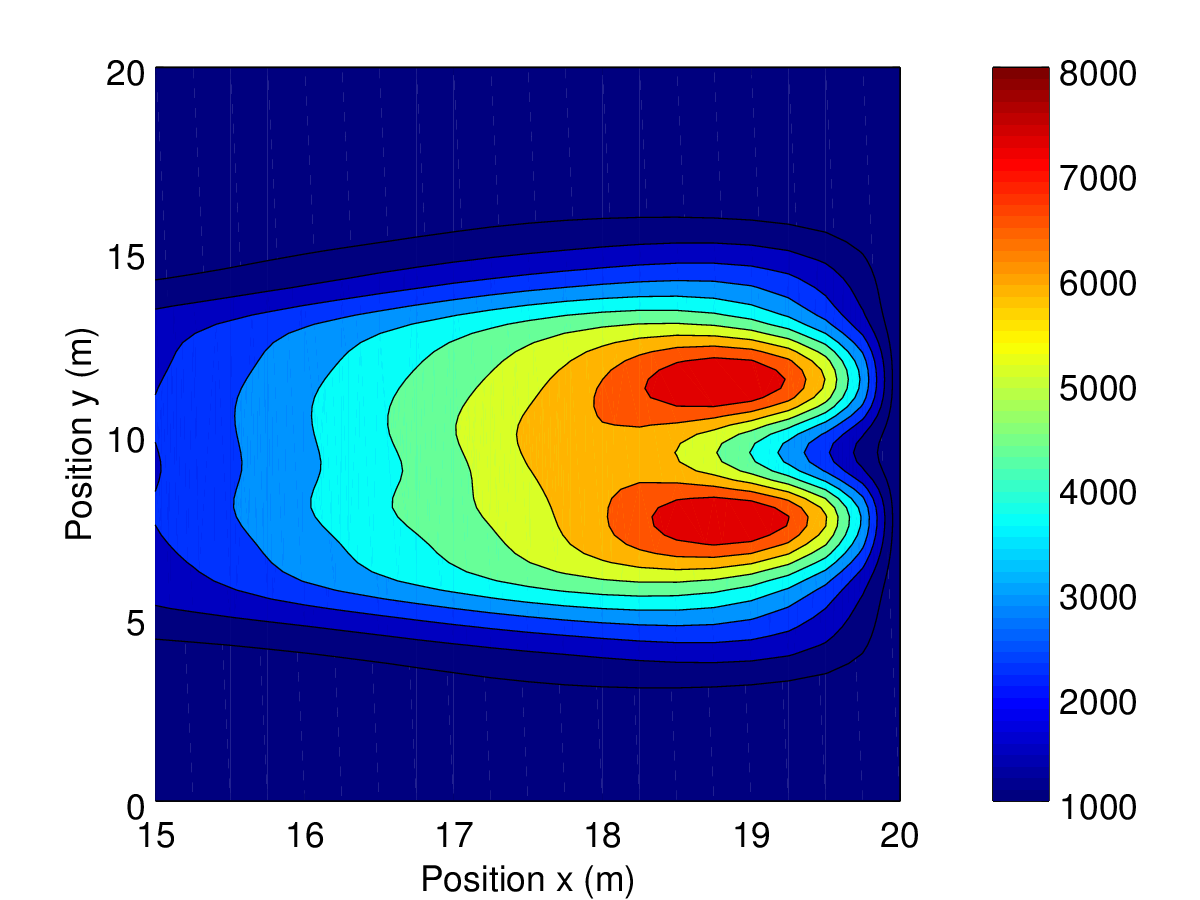
\includegraphics[height=5.5cm]{figuras/press_225p_v4_onedoor_3_6.png}
    \caption[width=5cm]{Isobaras cercanas a la puerta; la escala a la derecha está expresada en [PV]=N.m. La salida está centrada en la posición $x=20$~m e $y=10$~m y tiene ancho $L=3,6$~m. El recinto es de $20\times 20$~(m) con 225 individuos. La gráfica corresponde a valores medios a lo largo de 30 procesos de evacuación. Se usó un grillado de 1m$^2$ para promediar el campo de presiones (PV). La velocidad deseada de los individuos fue de $v_d=4$~m/s.}
    \label{isobaras_3_6m}
\end{figure}

\begin{figure}[H]
    \centering
    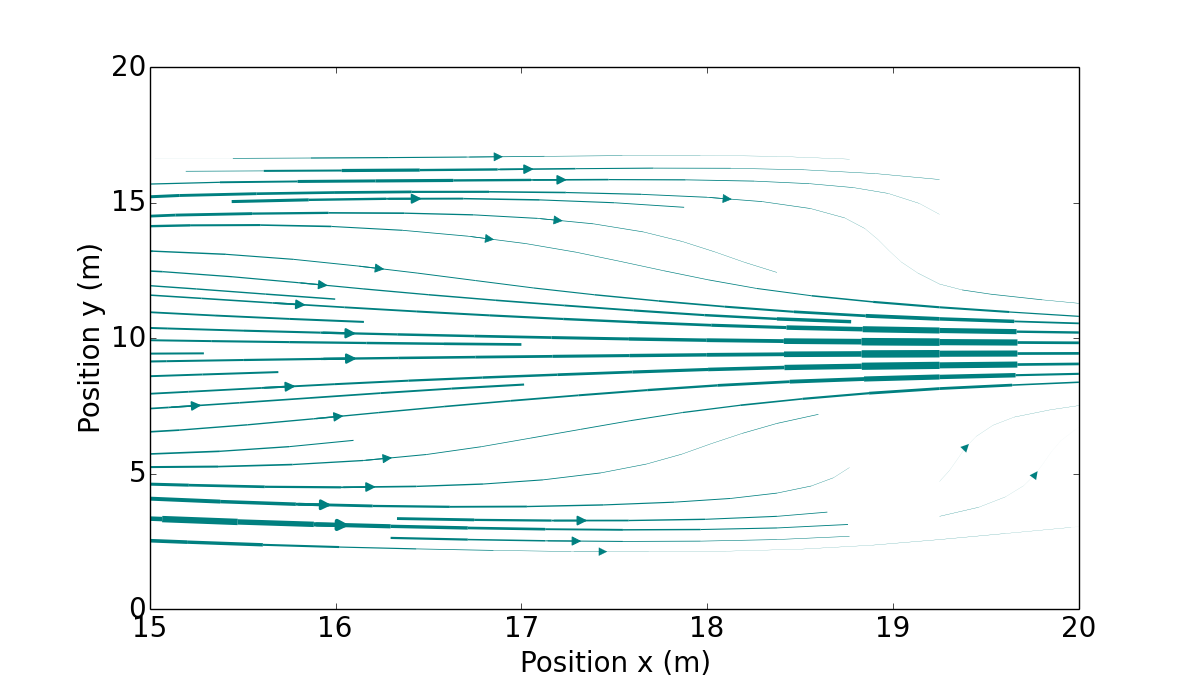
\includegraphics[height=5.5cm]{figuras/flujo_door_3_6m.png}
    \caption[width=5cm]{Gráfico de velocidad. La salida está centrada en la posición $x=20$~m e $y=10$~m y tiene ancho $L=3,6$~m. El recinto es de $20\times 20$~(m) con 225 individuos. La gráfica corresponde a valores medios a lo largo de 30 procesos de evacuación. Se usó un grillado de 1m$^2$ para promediar el campo de velocidades. La velocidad deseada de los individuos fue de $v_d=4$~m/s.}
    \label{sintesis}
\end{figure}

\begin{figure}[H]
    \centering
    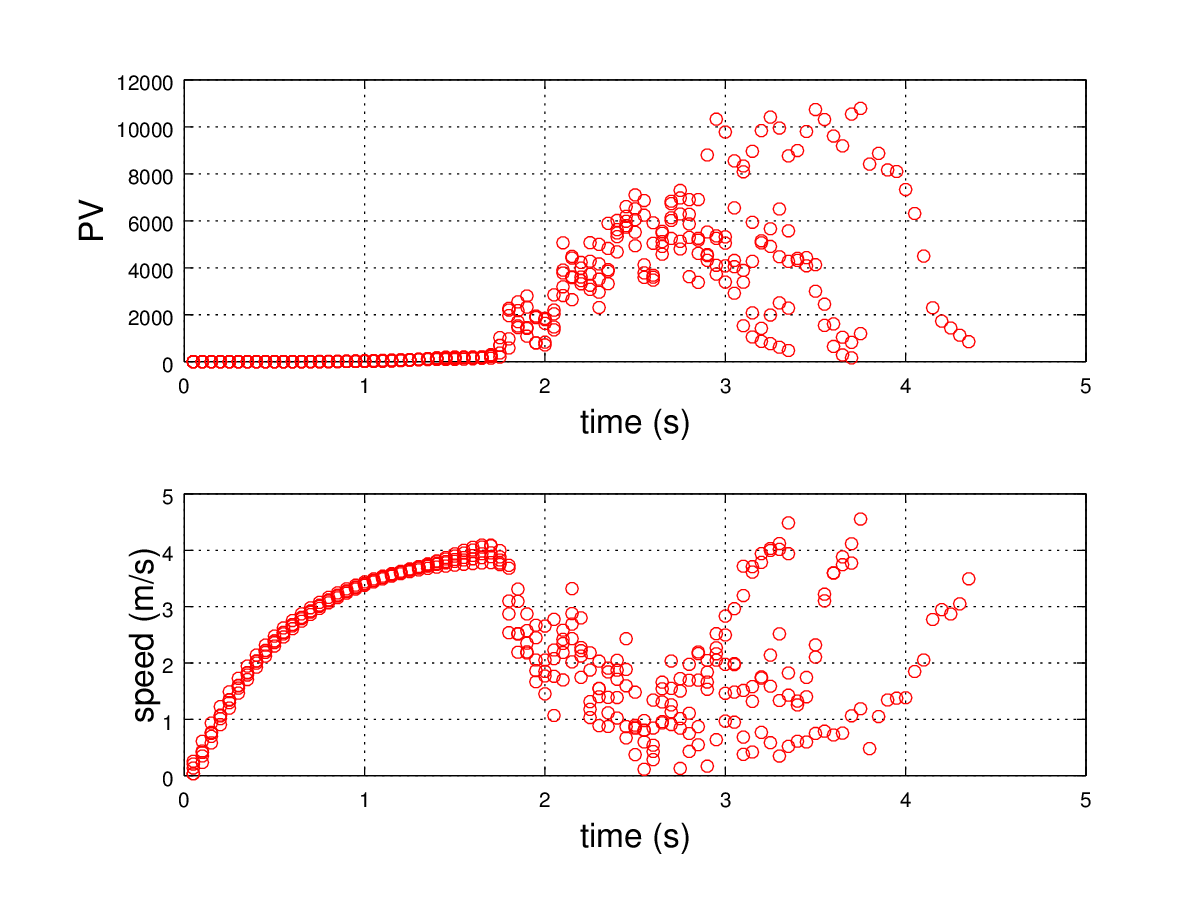
\includegraphics[height=5.5cm]{figuras/pv_vel_t_100_3_6.png}
    \caption[width=5cm]{Gráfico de velocidad(inferior) y presión(superior) en función del tiempo para un individuo ubicado inicialmente en $x=10$~m e $y=10$~m.  La salida está centrada en la posición $x=20$~m e $y=10$~m y tiene ancho $L=3,6$~m. El recinto es de $20\times 20$~(m) con 225 individuos. La gráfica corresponde a cinco iteraciones diferentes (variando la velocidad incial). La velocidad deseada del individuo fue de $v_d=4$~m/s.}
    \label{sintesis}
\end{figure}

\subsubsection{Puerta angosta (1,2 m)}

\begin{figure}[H]
    \centering
    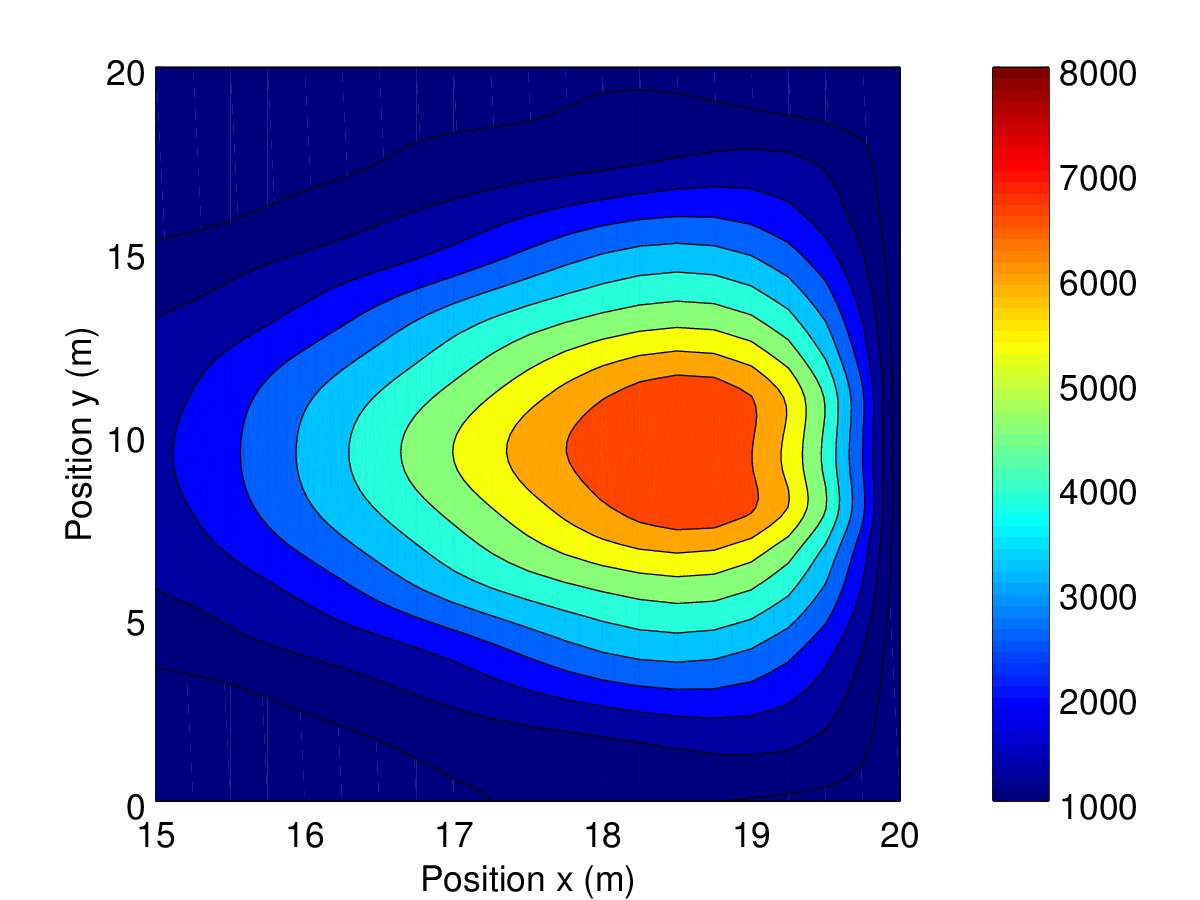
\includegraphics[height=5.5cm]{figuras/press_225p_v4_onedoor_1_2.png}
    \caption[width=5cm]{Isobaras cercanas a la puerta; la escala a la derecha está expresada en [PV]=N.m. La salida está centrada en la posición $x=20$~m e $y=10$~m y tiene ancho $L=1,2$~m. El recinto es de $20\times 20$~(m) con 225 individuos. La gráfica corresponde a valores medios a lo largo de 30 procesos de evacuación. Se usó un grillado de 1m$^2$ para promediar el campo de presiones (PV). La velocidad deseada de los individuos fue de $v_d=4$~m/s.}
    \label{isobaras_1_2m}
\end{figure}

\begin{figure}[H]
    \centering
    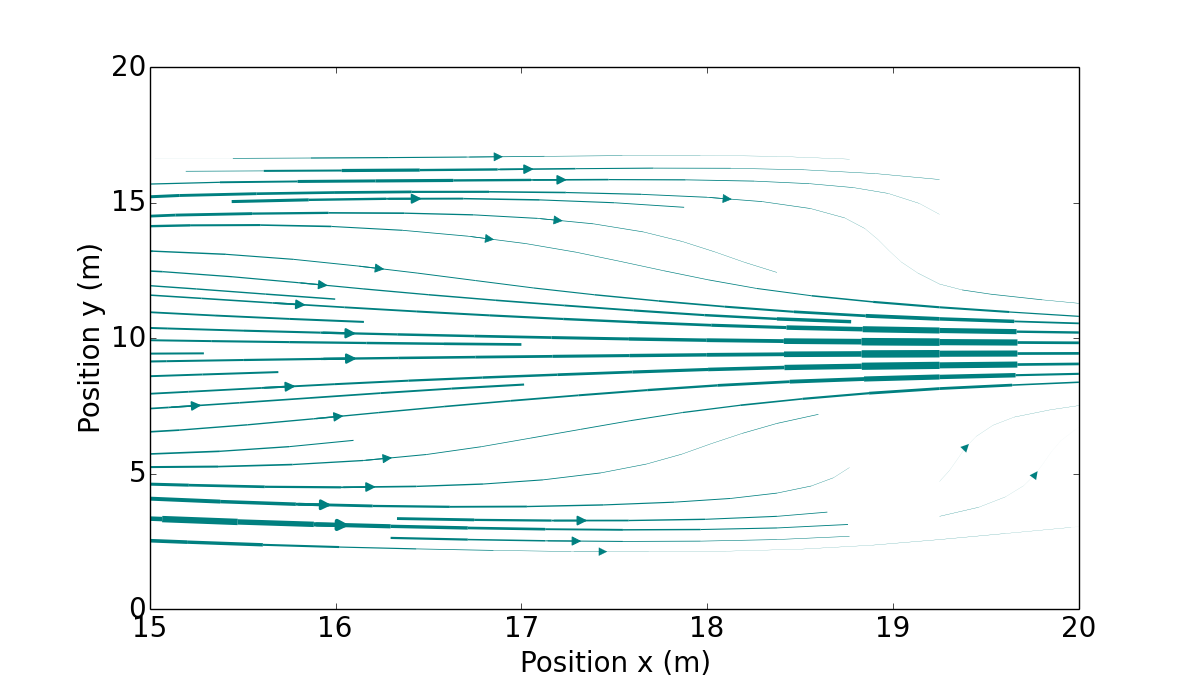
\includegraphics[height=5.5cm]{figuras/flujo_door_1_2m.png}
    \caption[width=5cm]{Gráfico de velocidad. La salida está centrada en la posición $x=20$~m e $y=10$~m y tiene ancho $L=1,2$~m. El recinto es de $20\times 20$~(m) con 225 individuos. La gráfica corresponde a valores medios a lo largo de 30 procesos de evacuación. Se usó un grillado de 1m$^2$ para promediar el campo de velocidades. La velocidad deseada de los individuos fue de $v_d=4$~m/s.}
    \label{sintesis}
\end{figure}

\begin{figure}[H]
    \centering
    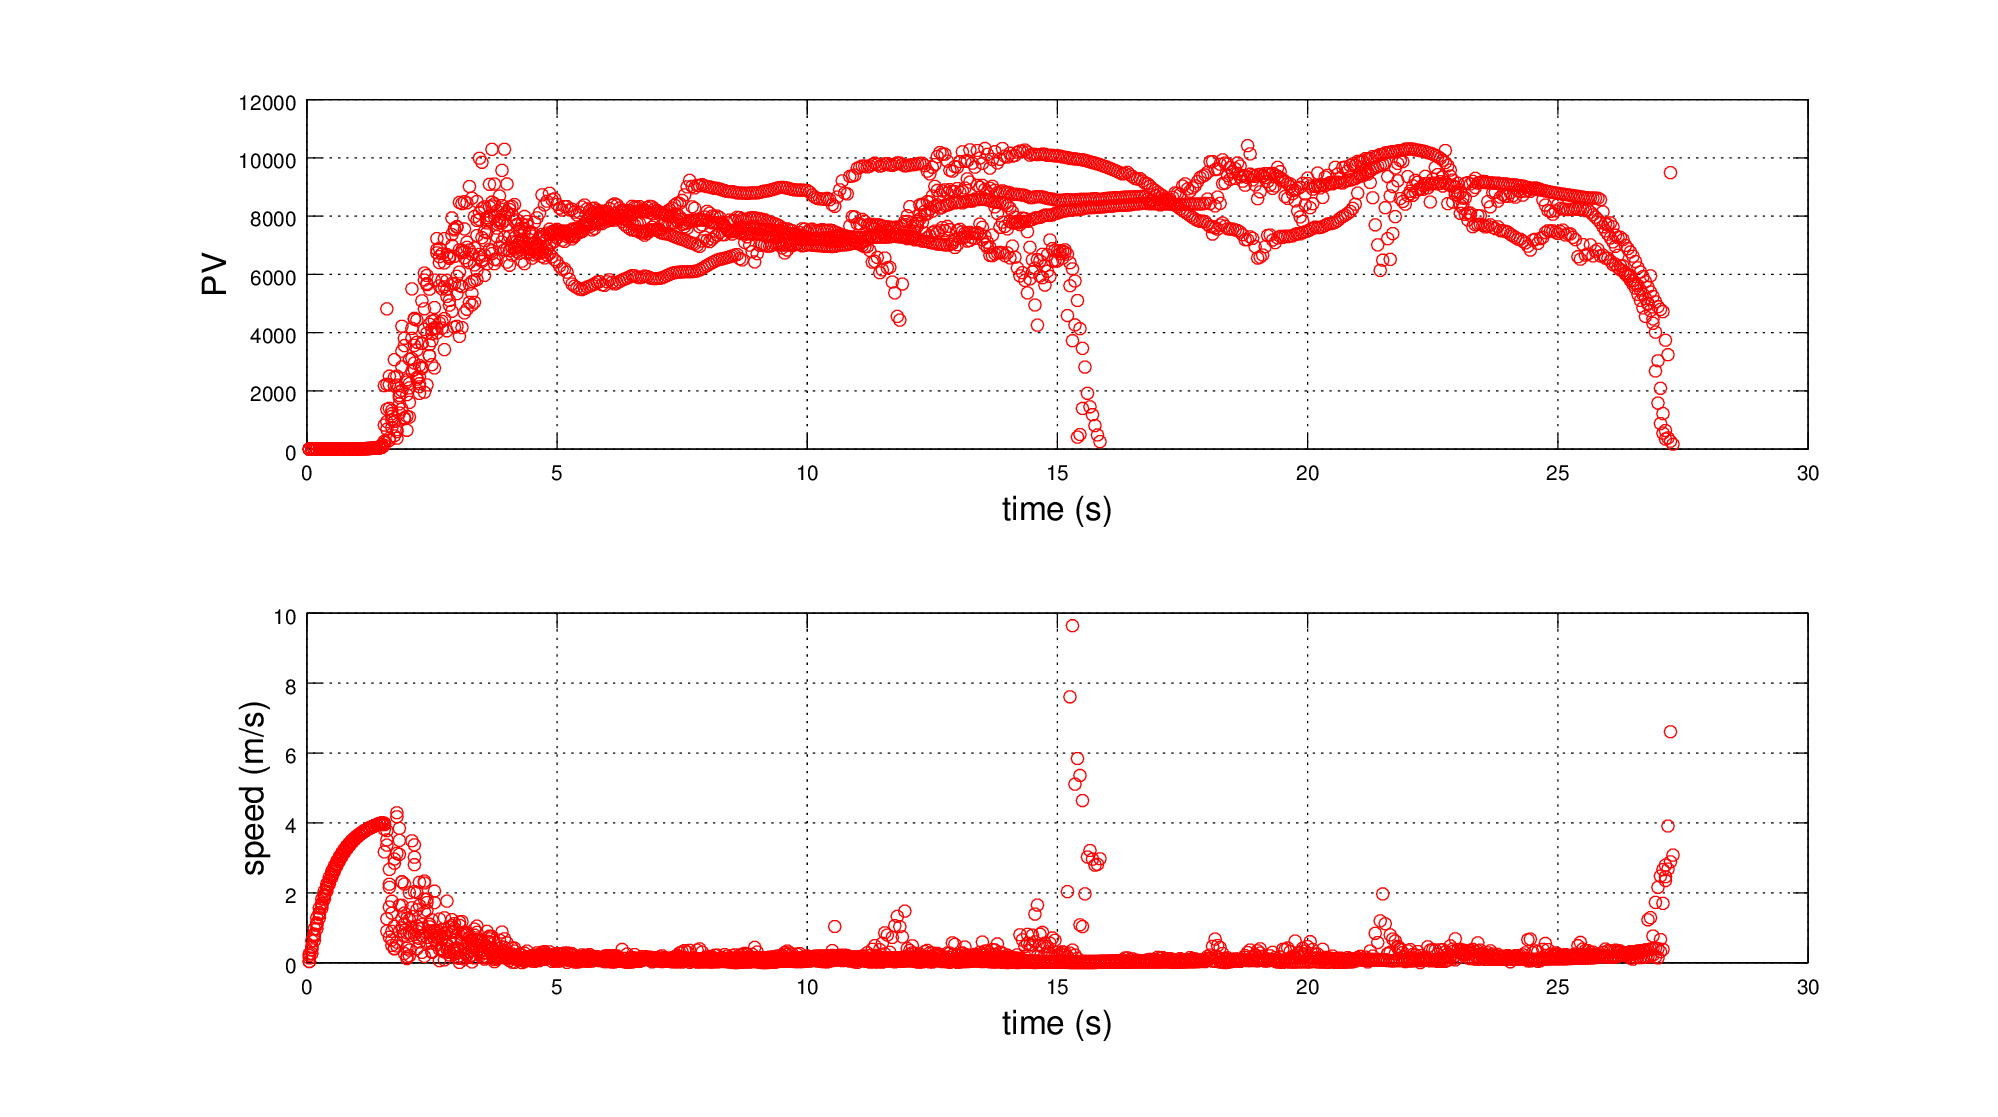
\includegraphics[height=5.5cm]{figuras/pv_vel_t_100_1_2.png}
    \caption[width=5cm]{Gráfico de velocidad(inferior) y presión(superior) en función del tiempo para un individuo ubicado inicialmente en $x=10$~m e $y=10$~m.  La salida está centrada en la posición $x=20$~m e $y=10$~m y tiene ancho $L=1,2$~m. El recinto es de $20\times 20$~(m) con 225 individuos. La gráfica corresponde a cinco iteraciones diferentes (variando la velocidad incial). La velocidad deseada del individuo fue de $v_d=4$~m/s.}
    \label{sintesis}
\end{figure}



\section{Dos puertas}

\subsection{Faster is slower}

\subsection{Tiempo de evacuación}

\begin{figure}[H]
    \centering
    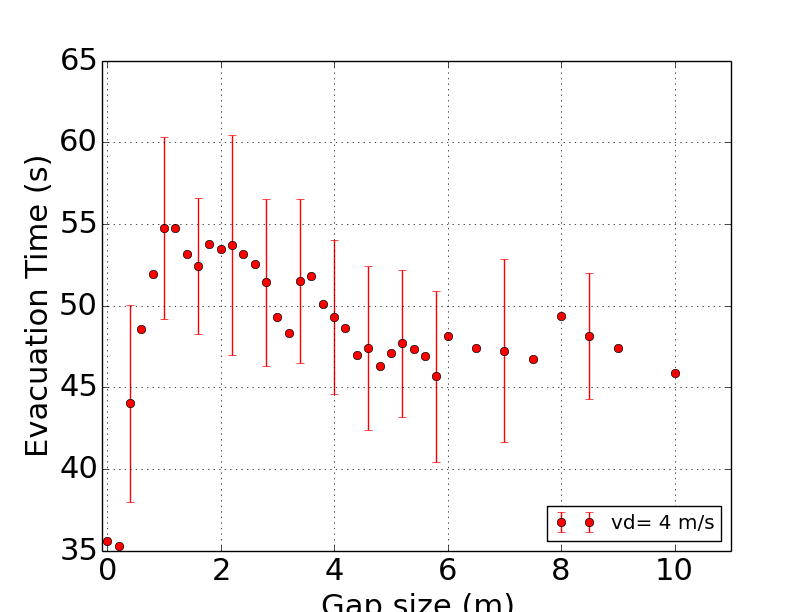
\includegraphics[height=5.5cm]{figuras/gap_vste_225p.png}
    \caption[width=5cm]{Gráfico de tiempo de evacuación en función del gap. El recinto es de $20\times 20$~(m) con 225 individuos y dos puertas, cada una tiene un ancho de $L=1,2$~m. La gráfica corresponde al promedio de treinta iteraciones. La velocidad deseada del individuo fue de $v_d=4$~m/s. Cada simulación termina cuando evacúan 160 individuos.}
    \label{sintesis}
\end{figure}

\begin{figure}[H]
    \centering
    \includegraphics[height=5.5cm]{figuras/gap_vsten.png}
    \caption[width=5cm]{Gráfico de tiempo de evacuación en función del gap para recintos de $20\times 20$~(m), $30\times 30$~(m) y $40\times 40$~(m) con 225, 580 y 961 individuos respectivamente. Todos los recintos tienen dos puertas, cada una de ancho $L=1,2$~m. Las gráficas corresponden al promedio de treinta iteraciones. Para todos los casos, la velocidad deseada del individuo fue de $v_d=4$~m/s. Cada simulación termina cuando evacúan 160, 529 y 961 individuos respectivamente.}
    \label{sintesis}
\end{figure}

\begin{figure}[H]
    \centering
    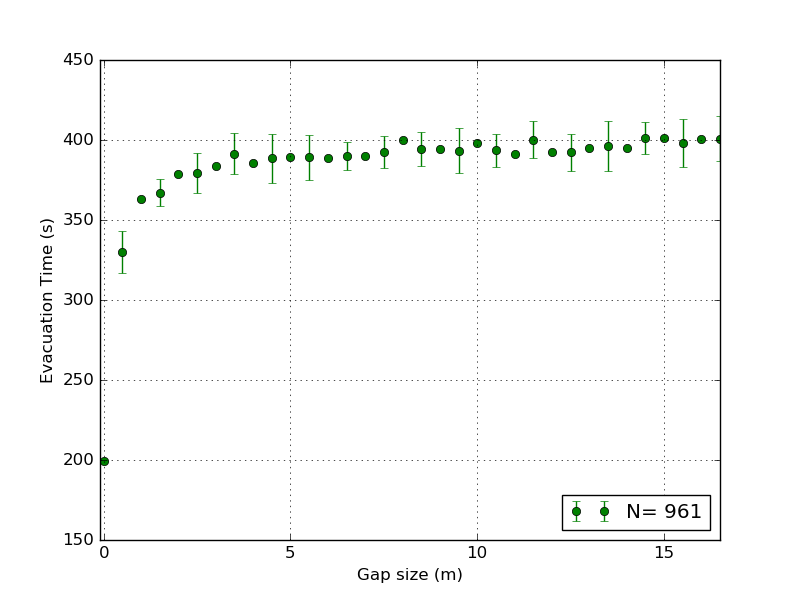
\includegraphics[height=5.5cm]{figuras/gap_vste_v4_961p.png}
    \caption[width=5cm]{Gráfico de tiempo de evacuación en función del gap. El recinto es de $40\times 40$~(m) con 961 individuos y dos puertas, cada una tiene un ancho de $L=1,2$~m. La gráfica corresponde al promedio de treinta iteraciones. La velocidad deseada del individuo fue de $v_d=4$~m/s. Cada simulación termina cuando evacúan 864 individuos.}
    \label{sintesis}
\end{figure}

\begin{figure}[H]
    \centering
    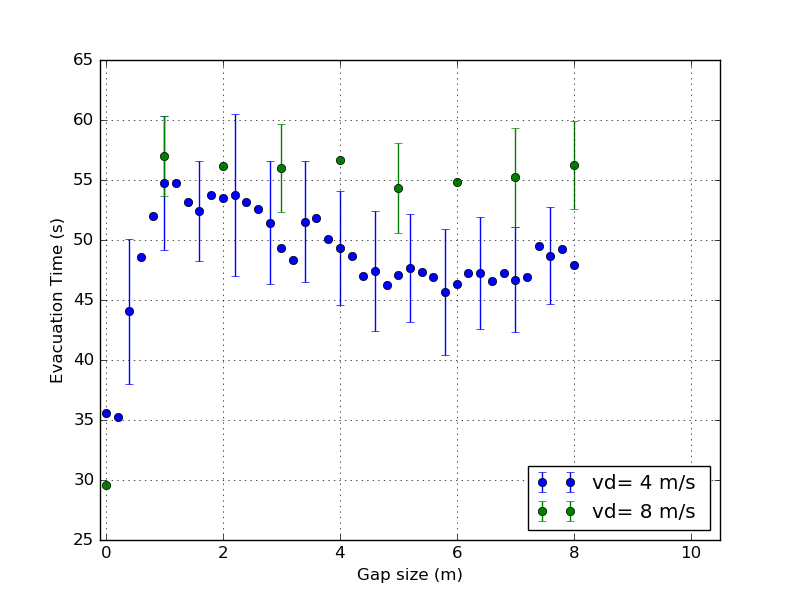
\includegraphics[height=5.5cm]{figuras/gap_vste_v4_v8.png}
    \caption[width=5cm]{Gráfico de tiempo de evacuación en función del gap. El recinto es de $20\times 20$~(m) con 225 individuos y dos puertas, cada una tiene un ancho de $L=1,2$~m. La gráfica corresponde al promedio de treinta iteraciones. Las velocidades de deseo de los individuos es de $v_d=4$~m/s y $v_d=8$~m/s. Cada simulación termina cuando evacúan 160 individuos.}
    \label{sintesis}
\end{figure}




\subsection{Blocking clusters}

\begin{figure}[H]
    \centering
    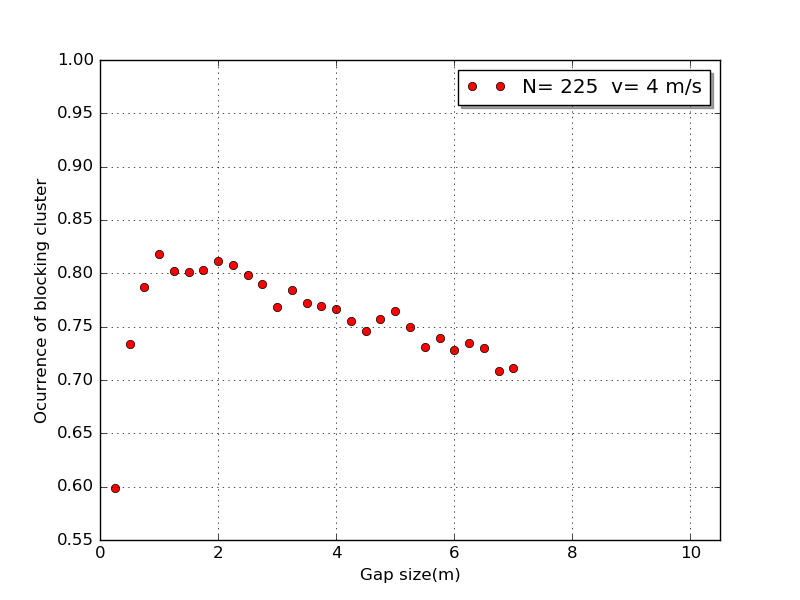
\includegraphics[height=5.5cm]{figuras/proba_vsgap_small_225p_v4.png}
    \caption[width=5cm]{Probabilidad de formar small blocking clusters (bloqueos de una sola puerta) en función del gap. El recinto es de $20\times 20$~(m) con 225 individuos y dos puertas, cada una tiene un ancho de $L=1,2$~m. La gráfica corresponde al promedio de treinta iteraciones. La velocidad de deseo es de $v_d=4$~m/s. Cada simulación termina cuando evacúan 160 individuos.}
    \label{sintesis}
\end{figure}

\begin{figure}[H]
    \centering
    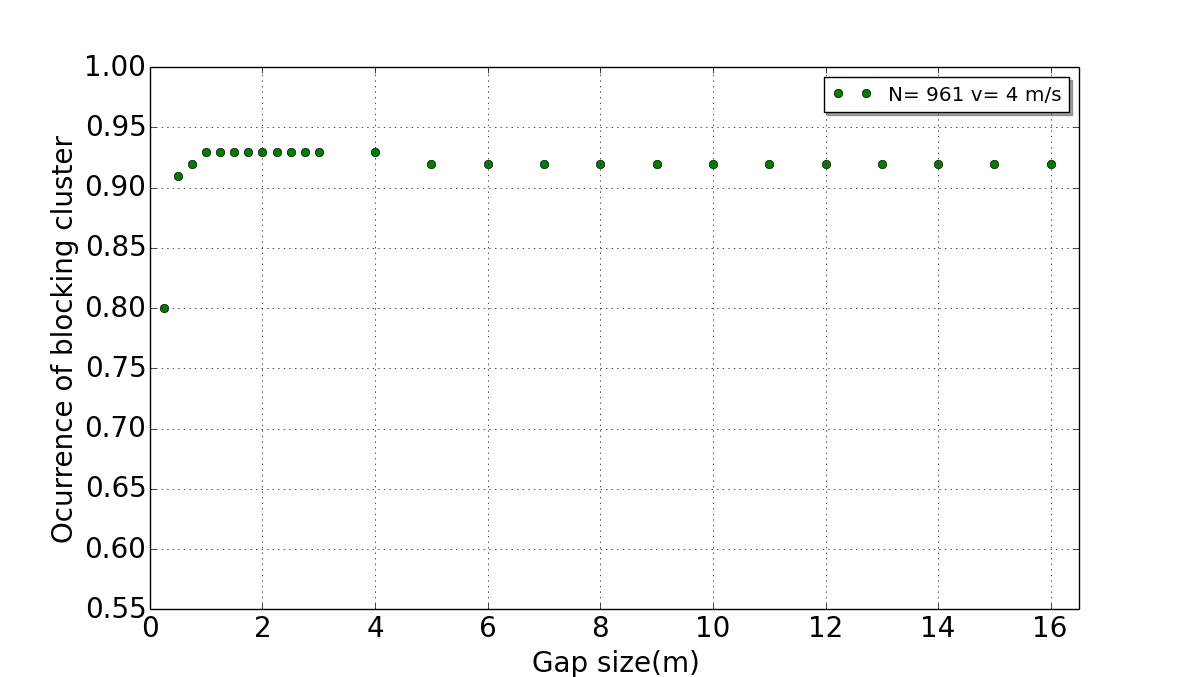
\includegraphics[height=5.5cm]{figuras/proba_vsgap_small_961p_v4.png}
    \caption[width=5cm]{Probabilidad de formar small blocking clusters (bloqueos de una sola puerta) en función del gap. El recinto es de $40\times 40$~(m) con 961 individuos y dos puertas, cada una tiene un ancho de $L=1,2$~m. La gráfica corresponde al promedio de treinta iteraciones diferentes. La velocidad de deseo es de $v_d=4$~m/s. Cada simulación termina cuando evacúan 864 individuos.}
    \label{sintesis}
\end{figure}

\begin{figure}[H]
    \centering
    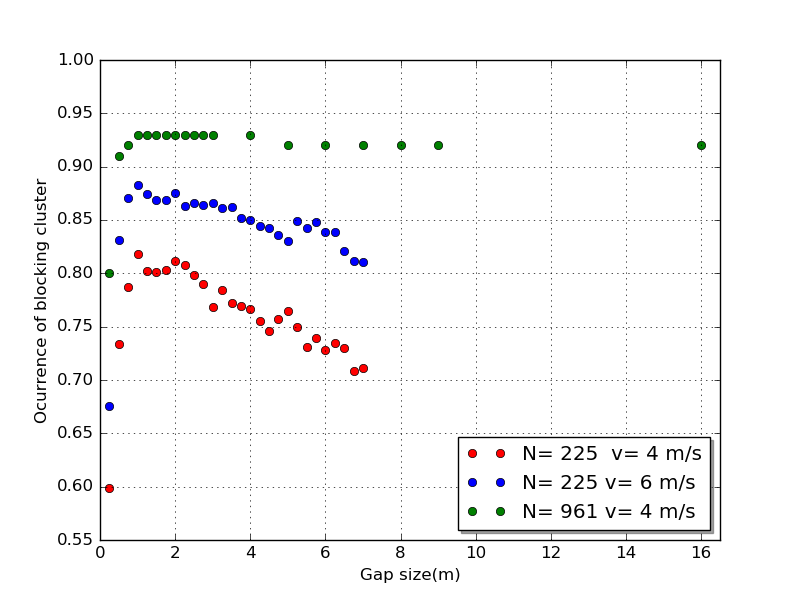
\includegraphics[height=5.5cm]{figuras/proba_vsgap_small_all.png}
    \caption[width=5cm]{Probabilidad de formar small blocking clusters (bloqueos de una sola puerta) en función del gap, para un recinto $20\times 20$~(m) con 225 individuos a $v_d=4$~m/s y $v_d=6$~m/s. Lo mismo para un recinto de $40\times 40$~(m) con 961 individuos a $v_d=4$~m/s. Ambos recintos poseén dos puertas, cada una tiene un ancho de $L=1,2$~m. Las gráficas corresponden al promedio de treinta iteraciones diferentes. Las simulación terminan cuando evacúan 160 individuos y 864 respectivamente.}
    \label{sintesis}
\end{figure}

\begin{figure}[H]
    \centering
    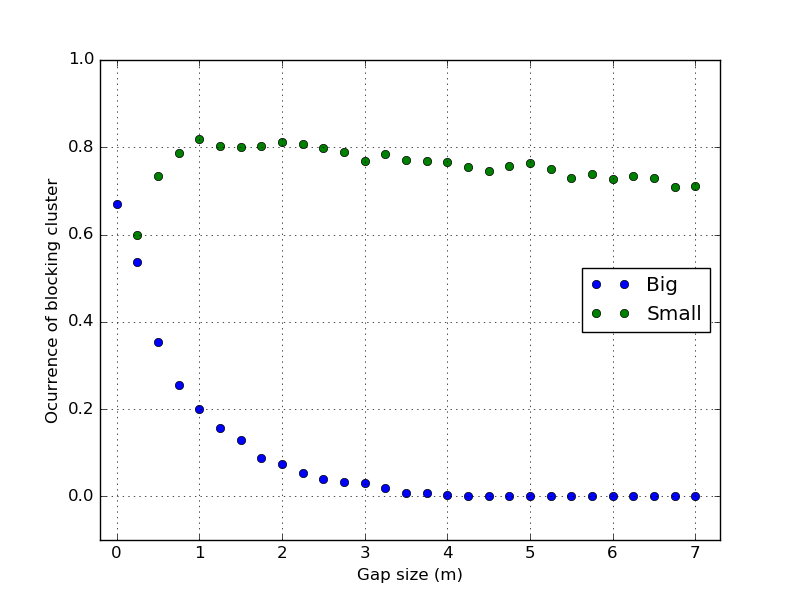
\includegraphics[height=5.5cm]{figuras/proba_vsgap_v4_big_small.png}
    \caption[width=5cm]{Probabilidad de formar big y small blocking clusters (bloqueos de dos y una puerta respectivamente) en función del gap. El recinto es de $20\times 20$~(m) con 225 individuos y dos puertas, cada una tiene un ancho de $L=1,2$~m. Las gráficas corresponden al promedio de treinta iteraciones diferentes. La velocidad de deseo es de $v_d=4$~m/s. Cada simulación termina cuando evacúan 160 individuos.}
    \label{sintesis}
\end{figure}



\subsection{Presión}

\begin{figure}[H]
    \centering
    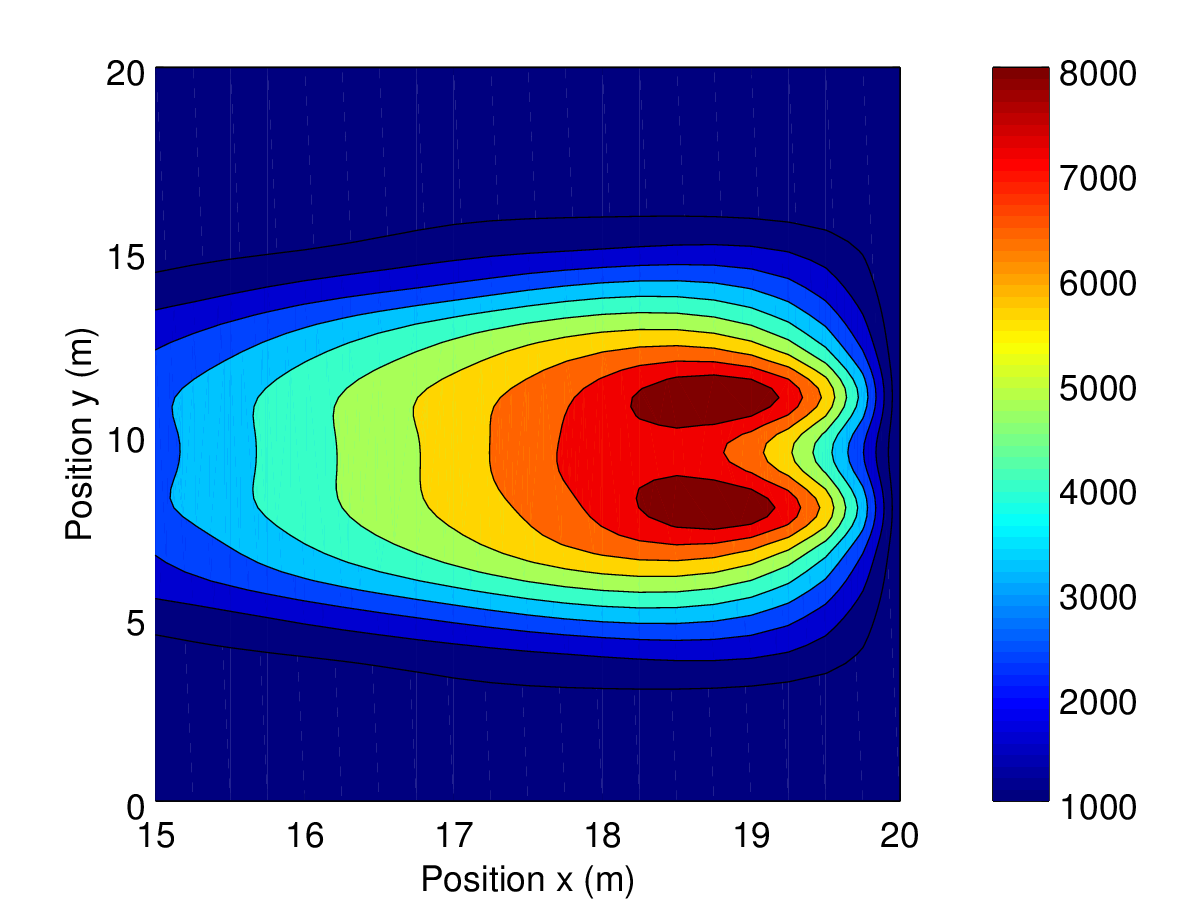
\includegraphics[height=5.5cm]{figuras/press_225p_v4_g0.png}
    \caption[width=5cm]{Isobaras cercanas a la puerta; la escala a la derecha está expresada en [PV]=N.m. La salida está centrada en la posición $x=20$~m e $y=10$~m, son dos puertas de ancho $L=1,2$~m con $g=0$~m. El recinto es de $20\times 20$~(m) con 225 individuos. La gráfica corresponde a valores medios a lo largo de 30 procesos de evacuación. Se usó un grillado de 1m$^2$ para promediar el campo de presiones (PV). La velocidad deseada de los individuos fue de $v_d=4$~m/s.}
    \label{presion_225p_g0}
\end{figure}

\begin{figure}[H]
    \centering
    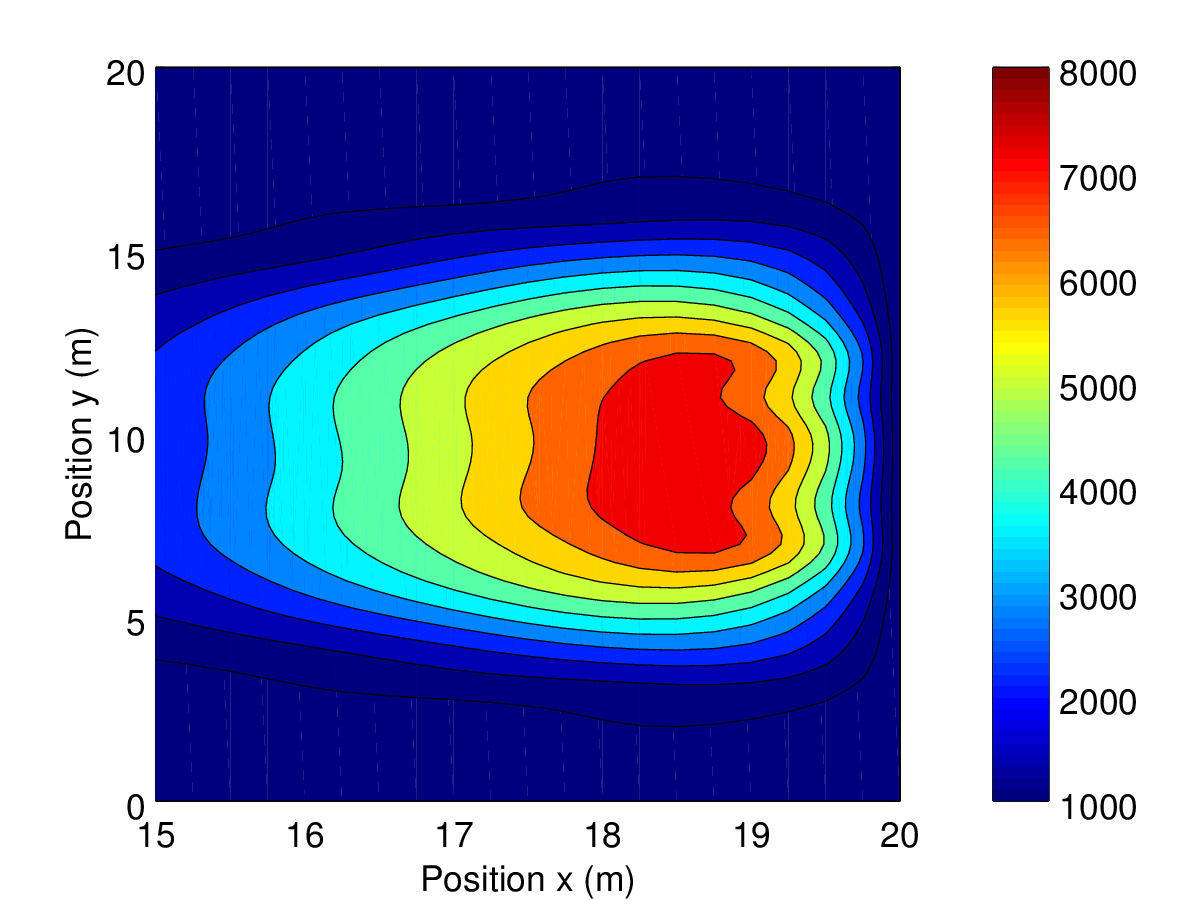
\includegraphics[height=5.5cm]{figuras/press_225p_v4_g1_5.png}
    \caption[width=5cm]{Isobaras cercanas a la puerta; la escala a la derecha está expresada en [PV]=N.m. La salida consta de dos puertas de ancho $L=1,2$~m separadas entre si por una distancia de $g=1,5$~m, centrdas en $x=20$~m e $y=11,35$~m y $x=20$~m e $y=8,65$~m . El recinto es de $20\times 20$~(m) con 225 individuos. La gráfica corresponde a valores medios a lo largo de 30 procesos de evacuación. Se usó un grillado de 1m$^2$ para promediar el campo de presiones (PV). La velocidad deseada de los individuos fue de $v_d=4$~m/s.}
    \label{presion_225p_g1_5}
\end{figure}

\begin{figure}[H]
    \centering
    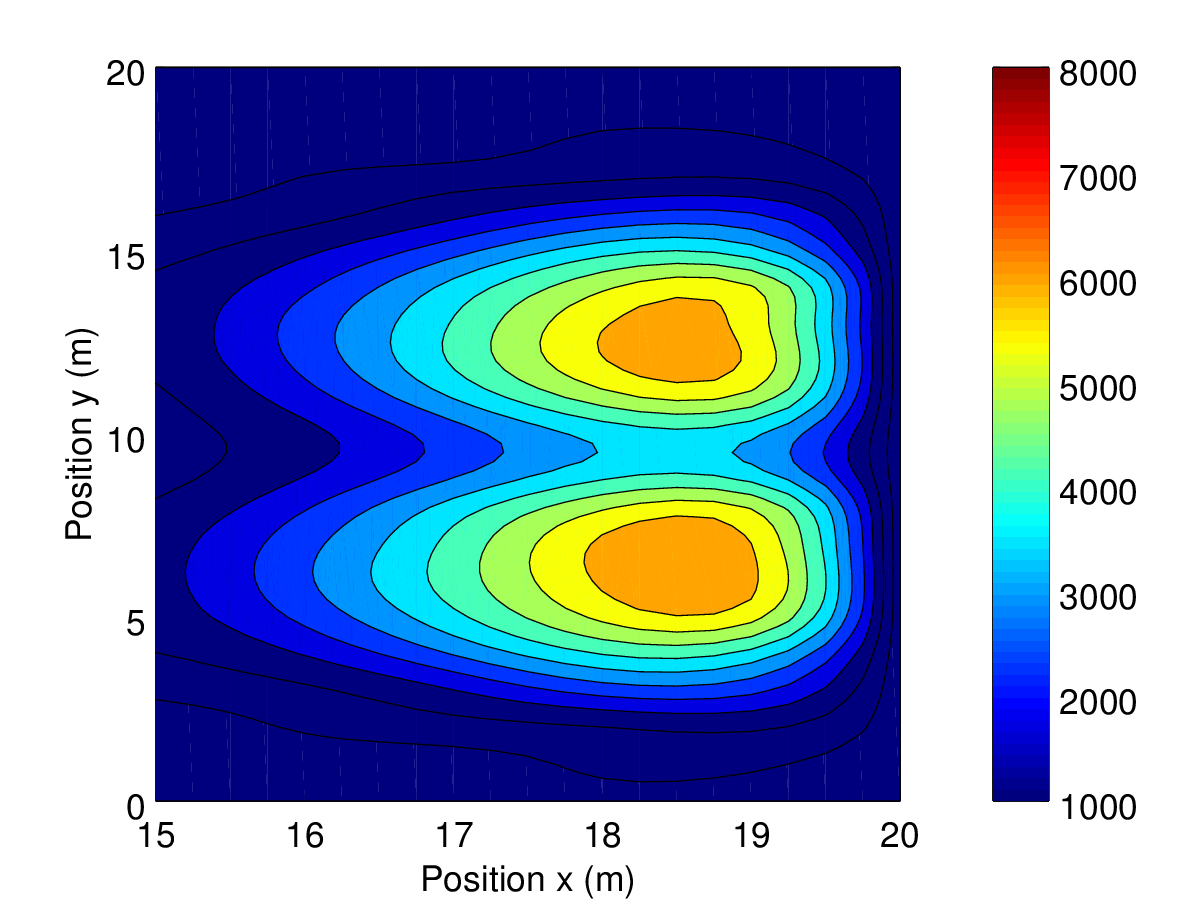
\includegraphics[height=5.5cm]{figuras/press_225p_v4_g5.png}			\caption[width=5cm]{Isobaras cercanas a la puerta; la escala a la derecha está expresada en [PV]=N.m. La salida consta de dos puertas de ancho $L=1,2$~m separadas entre si por una distancia de $g=1,5$~m, centrdas en $x=20$~m e $y=12,5$~m y $x=20$~m e $y=7,5$~m. El recinto es de $20\times 20$~(m) con 225 individuos. La gráfica corresponde a valores medios a lo largo de 30 procesos de evacuación. Se usó un grillado de 1m$^2$ para promediar el campo de presiones (PV). La velocidad deseada de los individuos fue de $v_d=4$~m/s.}
    \label{presion_225p_g5}
\end{figure}




%\subsection{Velocidad}
\subsection{Comportamiento asintótico}





\chapter{Conclusiones}
En este trabajo de tesis se implementaron códigos que permitieron realizar simulaciones de multitudes evacuando en estado de pánico según el modelo de fuerza social. \\

Para recintos con una única salida se obtuvieron dinámicas diferentes según el tamaño de la puerta. Si esta es ancha, el flujo de evacuación es permanente (\emph{i.e.} prácticamente no hay momentos en los que todos los peatones se encuentren sin poder moverse). Las zonas de mayor presión se dan a los costados de la puerta. Cuando la salida es angosta la evacuación es intermitente (\emph{i.e.} por momentos algunos peatones logran salir y en otras ocasiones todos están quietos); este efecto de Stop-and-go hace que la zona de máxima presión se de en el medio del bulk (dos metros antes de la puerta aproximadamente). 
Para ambos recintos la mayor velocidad de los individuos se tiene en el medio. \\

En cuanto a los recintos con dos puertas en un mismo lado, se obtuvo  una separación crítica para la cual cambia la pendiente de la curva tiempo de evacuación vs. separación (gap). Este valor es $g_c=1,5$~m y coincide aproximadamente con el ancho de dos peatones. Esta cantidad es independiente del número de individuos y la velocidad de deseo. Esto permitió afirmar que el $g_c$ afecta a los bloqueos que ocurren en las cercanías de la salida. \\

La forma funcional de la probabilidad de formar small blocking clusters es similar a la forma funcional del tiempo de evacuación, esto denota que los bloqueos de cada una de las puertas son determinantes en la eficiencia de la evacuación. \\

Aumentar el nivel de ansiedad de los individuos mediante la velocidad de deseo genera evacuaciones más lentas así como aumentar la cantidad de individuos en el recinto. Esto coincide con los resultados obtenidos de la presión que soportan los individuos del blocking cluster. En todos los casos aumentar $v_d$ o N genera un incremento de la presión y tiene como consecuencia evacuaciones menos eficientes.\\

El mejor rendimiento en las evacuaciones se dio cuando las puertas no tienen separación entre sí ($g=0$~m). Separar la salida en dos puertas empeora el rendimiento a pesar de que la apertura total tenga el mismo tamaño. Pero, si por razones estructurales hay que construir dos puertas lo mejor es hacerlo dejando una distancia de separación de por lo menos 6~m (bajo las condiciones de estudio de este trabajo).    

\bibliographystyle{plain} %Choose a bibliograhpic style
\bibliography{bibliografia/biblio}



\end{document}